\subsection{Quicksort Results:}

\subsubsection{Worst case:}

First test for {\bfseries\itshape Quicksort}. The program will plot the {\bfseries\itshape time} that the algorithm takes to sort a list of length {\bfseries\itshape n = 6}. \hfill \break

{\bfseries\itshape\color{armygreen}{Observation:}} {\itshape\color{armygreen}{We are going to analyze the worst case when the list it's sorted in decreasing order.}} \hfill \break

\begin{figure}[H]
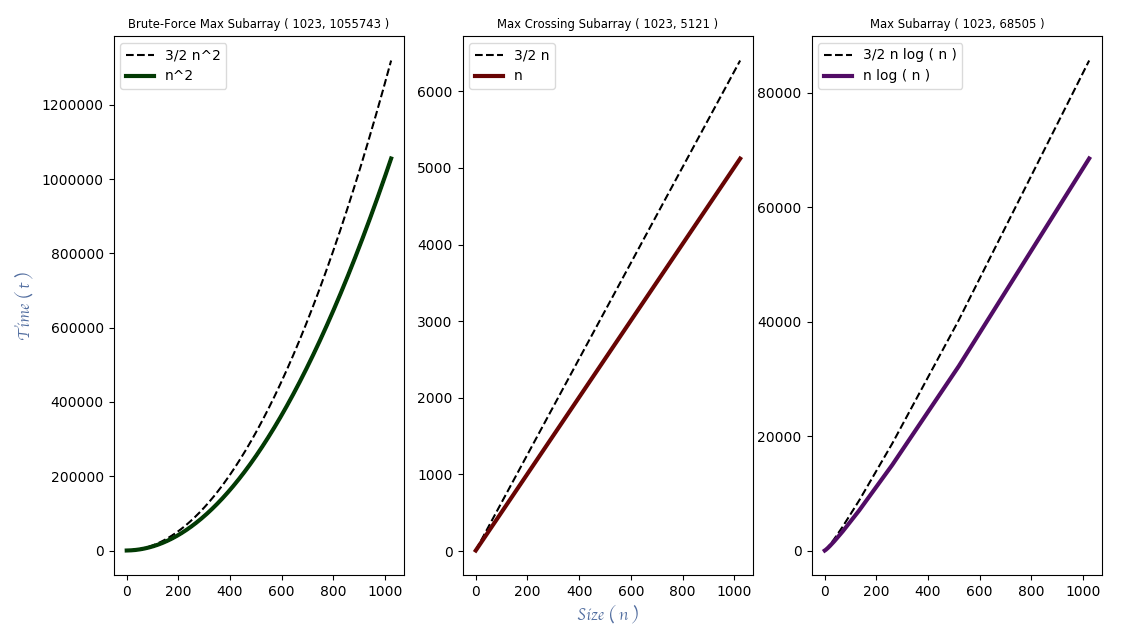
\includegraphics[scale=.54]{t1.png}
\centering \linebreak \linebreak Figure 4.1.1.0: Testing Quicksort with a list of length n = 6.
\end{figure} \hfill 

\begin{multicols}{2}
\begin{figure}[H]
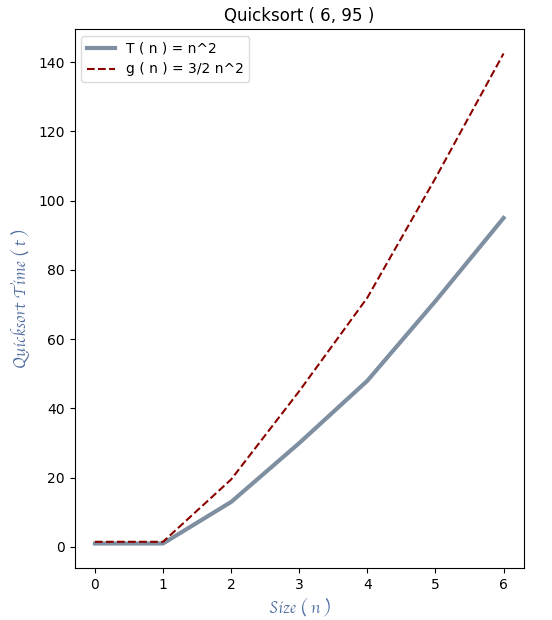
\includegraphics[scale=.5]{p1.png}
\centering \linebreak \linebreak Figure 4.1.1.1: Graph for Figure 4.1.1.0.
\end{figure} \hfill

\begin{center}
\begin{itemize}

\end{itemize}
{\Large
\begin{tabular}[.5cm]{ c c c }
\toprule
Length ( n ) & Time ( t ) \\
\midrule
0 & 1 \\
\cmidrule {1-2}
1 & 2 \\
\cmidrule {1-2}
2 & 13 \\
\cmidrule {1-2}
3 & 30 \\
\cmidrule {1-2}
4 & 48 \\
\cmidrule {1-2}
5 & 71 \\
\cmidrule {1-2}
6 & 95 \\
\bottomrule
\linebreak
\end{tabular}}
\linebreak \linebreak Table 1: Plot point for Figure 4.1.1.1.
\end{center}
\end{multicols}

\pagebreak

Second test for {\bfseries\itshape Quicksort}. The program will plot the {\bfseries\itshape time} that the algorithm takes to sort a list of length {\bfseries\itshape n = 20}. \hfill \break

{\bfseries\itshape\color{armygreen}{Observation:}} {\itshape\color{armygreen}{We are going to analyze another worst case when the list it's sorted in decreasing order.}} \hfill \break

\begin{figure}[H]
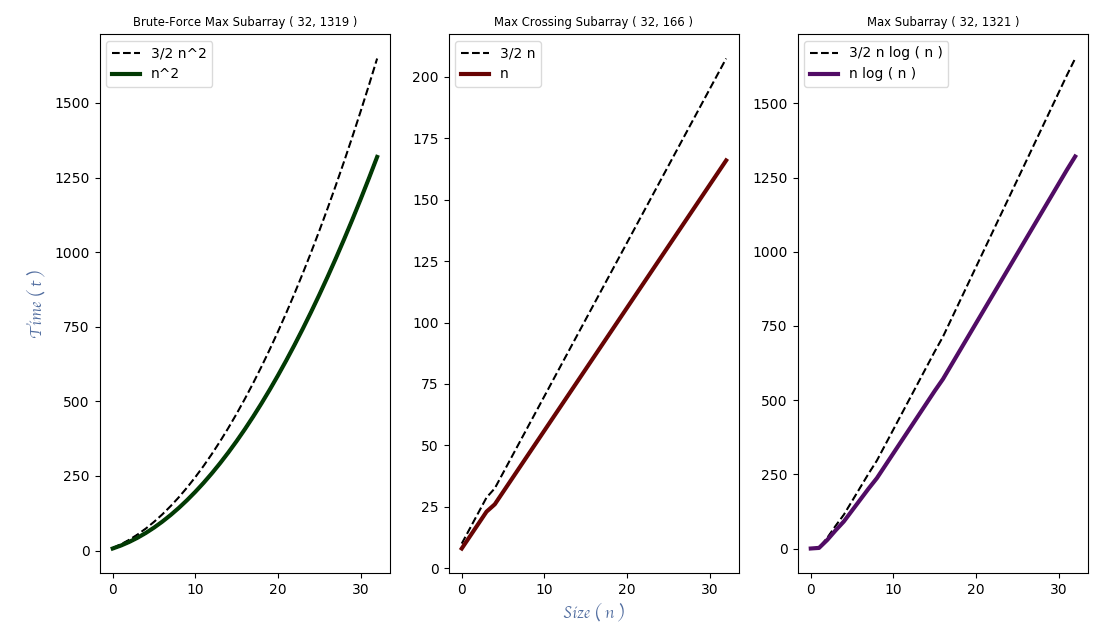
\includegraphics[scale=.54]{t2.png}
\centering \linebreak \linebreak Figure 4.1.1.2: Testing Quicksort with a list of length n = 20.
\end{figure} \hfill

\begin{multicols}{2}
\begin{figure}[H]
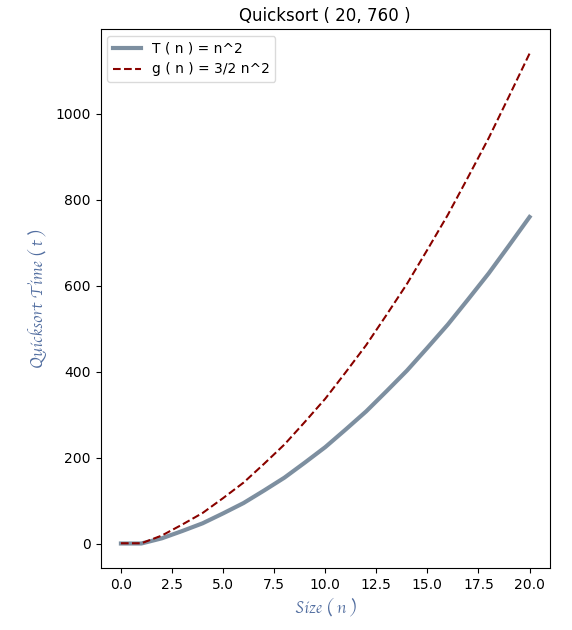
\includegraphics[scale=.5]{p2.png}
\centering \linebreak \linebreak Figure 4.1.1.3: Graph for Figure 4.1.1.2.
\end{figure}

\begin{center}
\begin{itemize}

\end{itemize}
\begin{tabular}[.5cm]{ c c c }
\toprule
Length ( n ) & Time ( t ) \\
\midrule
0 & 1 \\
\cmidrule {1-2}
1 & 2 \\
\cmidrule {1-2}
2 & 13 \\
\cmidrule {1-2}
3 & 30 \\
\cmidrule {1-2}
4 & 48 \\
\cmidrule {1-2}
5 & 71 \\
\cmidrule {1-2}
6 & 95 \\
\cmidrule {1-2}
7 & 124 \\
\cmidrule {1-2}
8 & 154 \\
\cmidrule {1-2}
9 & 189 \\
\cmidrule {1-2}
10 & 225 \\
\cmidrule {1-2}
11 & 266 \\
\cmidrule {1-2}
12 & 308 \\
\cmidrule {1-2}
13 & 355 \\
\cmidrule {1-2}
14 & 403 \\
\cmidrule {1-2}
15 & 456 \\
\cmidrule {1-2}
16 & 510 \\
\cmidrule {1-2}
17 & 569 \\
\cmidrule {1-2}
18 & 629 \\
\cmidrule {1-2}
19 & 694 \\
\cmidrule {1-2}
20 & 760 \\
\bottomrule
\linebreak
\end{tabular}
\linebreak \linebreak Table 2: Plot point for Figure 4.1.1.3.
\end{center}
\end{multicols} \hfill

{\bfseries\itshape\color{armygreen}{Observation:}} {\itshape\color{armygreen}{The {\bfseries red} graph represents our proposed function for the worst case of {\bfseries Quicksort} and the {\bfseries blue} one it's the temporal complexity.}} \hfill \break

{\bfseries\itshape\color{armygreen}{Observation:}} {\itshape\color{armygreen}{The function proposed is: {\bfseries g( n ) = ( 3/2 ) $n^{2}$}. }} \hfill \break

\pagebreak

\subsubsection{Random case:}

Third test for {\bfseries\itshape Quicksort}. The program will plot the {\bfseries\itshape time} that the algorithm takes to sort a list of length {\linebreak\bfseries\itshape n = 10}. \hfill \break

\begin{figure}[H]
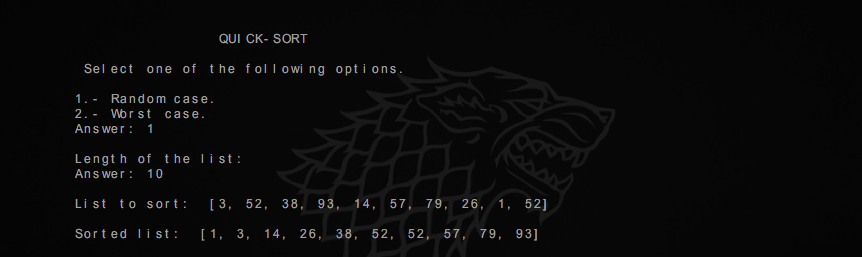
\includegraphics[scale=.54]{t3.png}
\centering \linebreak \linebreak Figure 4.1.2.0: Testing Quicksort with a list of length n = 10.
\end{figure} \hfill 

\begin{multicols}{2}
\begin{figure}[H]
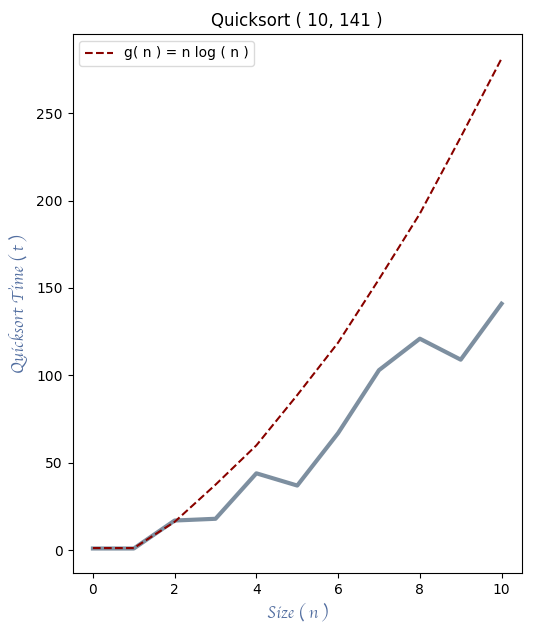
\includegraphics[scale=.5]{p3.png}
\centering \linebreak \linebreak Figure 4.1.2.1: Graph for Figure 4.1.2.0.
\end{figure} \hfill

\begin{center}
\begin{tabular}[.5cm]{ c c c }
\toprule
Length ( n ) & Time ( t ) \\
\midrule
0 & 1 \\
\cmidrule {1-2}
1 & 1 \\
\cmidrule {1-2}
2 & 17 \\
\cmidrule {1-2}
3 & 18 \\
\cmidrule {1-2}
4 & 44 \\
\cmidrule {1-2}
5 & 37 \\
\cmidrule {1-2}
6 & 67 \\
\cmidrule {1-2}
7 & 103 \\
\cmidrule {1-2}
8 & 121 \\
\cmidrule {1-2}
9 & 109 \\
\cmidrule {1-2}
10 & 141 \\
\bottomrule
\linebreak
\end{tabular}
\linebreak \linebreak Table 3: Plot point for Figure 4.1.2.1.
\end{center}
\end{multicols}

\pagebreak

Fourth test for {\bfseries\itshape Quicksort}. The program will plot the {\bfseries\itshape time} that the algorithm takes to sort a list of length {\bfseries\itshape n = 15}. \hfill \break

\begin{figure}[H]
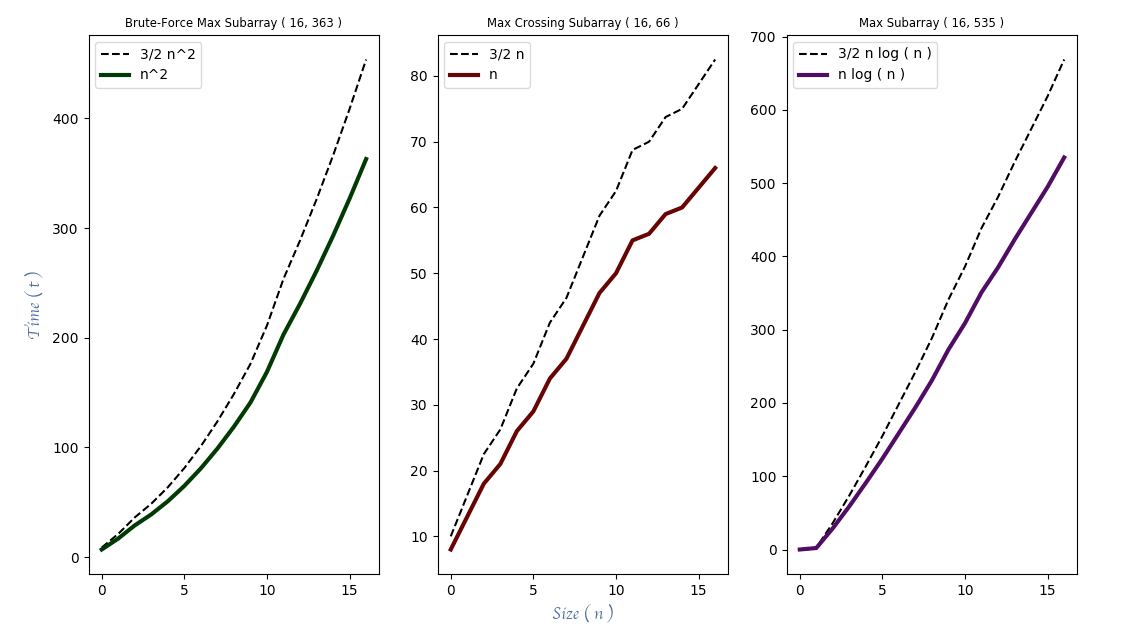
\includegraphics[scale=.54]{t4.png}
\centering \linebreak \linebreak Figure 4.1.2.2: Testing Quicksort with a list of length n = 15.
\end{figure} \hfill 

\begin{multicols}{2}
\begin{figure}[H]
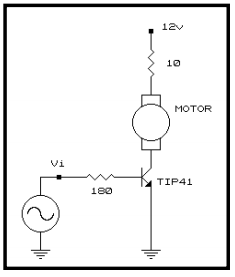
\includegraphics[scale=.5]{p4.png}
\centering \linebreak \linebreak Figure 4.1.2.3: Graph for Figure 4.1.2.2.
\end{figure} \hfill

\begin{center}
\begin{tabular}[.5cm]{ c c c }
\toprule
Length ( n ) & Time ( t ) \\
\midrule
0 & 1 \\
\cmidrule {1-2}
1 & 1 \\
\cmidrule {1-2}
2 & 13 \\
\cmidrule {1-2}
3 & 18 \\
\cmidrule {1-2}
4 & 39 \\
\cmidrule {1-2}
5 & 70 \\
\cmidrule {1-2}
6 & 59 \\
\cmidrule {1-2}
7 & 80 \\
\cmidrule {1-2}
8 & 120 \\
\cmidrule {1-2}
9 & 127 \\
\cmidrule {1-2}
10 & 183 \\
\cmidrule {1-2}
11 & 154 \\
\cmidrule {1-2}
12 & 162 \\
\cmidrule {1-2}
13 & 181 \\
\cmidrule {1-2}
14 & 206 \\
\cmidrule {1-2}
15 & 281 \\
\bottomrule
\linebreak
\end{tabular}
\linebreak \linebreak Table 4: Plot point for Figure 4.1.2.3.
\end{center}
\end{multicols} \hfill \break

{\bfseries\itshape\color{armygreen}{Observation:}} {\itshape\color{armygreen}{The {\bfseries red} graph represents our proposed function for any other case of {\bfseries Quicksort} and the {\bfseries blue} one it's the temporal complexity.}} \hfill \break

{\bfseries\itshape\color{armygreen}{Observation:}} {\itshape\color{armygreen}{The function proposed is: {\bfseries g( n ) = n log ( n )}. }} \hfill \break

\pagebreak